\documentclass[a4j]{jarticle}

\usepackage[dvipdfmx]{graphicx}
\usepackage{amssymb}
\usepackage{subfigure}

\begin{document}
 AWS サーバもしくは SINET のウェブサーバを対象にした 15 秒周期での計測実験によって得られた区間データに対する実測値の系列および変動値の系列のうち,定常性を満たさない時系列データの数を ADF 検定をもとに求めた結果を使用言語別に表 1 に示します.ADF 検定とは,帰無仮説を定常性を満たさない, 対立仮説を定常性を満たすとした検定です.
 \begin{table}[tb]
 \centering
 \caption{定常性を満たさない時系列データの数(有意水準 5 \%)}
 \begin{tabular}{|c||c|c|c|c|}
 \hline
 & \multicolumn{2}{|c|}{{\bf AWS サーバに対する計 122 区間データ}} & \multicolumn{2}{|c|}{{\bf SINET ウェブサーバに対する計 98 区間データ}}\\
 \cline{2-5}
 & {\bf \hspace{1cm}実測値\hspace{1cm}} & {\bf 変動値} & {\bf \hspace{1cm}実測値\hspace{1cm}} & {\bf 変動値}\\
 \hline
 \hline
 {\bf R} & 0 & 0 & 9 & 0\\
 \hline
 {\bf python} & 3 & 0 & 13 & 0\\
 \hline
 \end{tabular}
 \end{table}
表 1 より,AWS サーバを対象とした計測データの実測値と変動値はともに, R 言語の ADF 検定より定常性を満たしていることがわかりました.
しかし,python の ADF 検定では実測値が定常性を満たしているとは言えませんでした.
詳しくは分からなかったのですが,python の方が ADF 検定の条件が厳しいと思われます.
 SINET のウェブサーバを対象としたものでも同様の傾向が見受けられました.
  
また,SINET のウェブサーバを対象とした計測データの実測値は R 言語の ADF 検定であっても,定常性を満たしているとは言えませんでした.
 AWS サーバと SINET のウェブサーバとの間に見られるこの違いは,図 1 に示すように,最小応答遅延時間と考えられる応答遅延がスパイク状になっているかどうかに起因すると思われます.

実測値の系列が定常性を満たすかどうかは,対象とするサーバによるところがあることが明らかになりました.SINET のウェブサーバの実測値のように応答遅延が最小応答遅延に近い位置で変動するものに関しては,時系列モデルによる回帰を行う際には変動値を用いるべきだと思われます.また,このような変動をするのは,ネットワーク内の帯域が大きかったりアクセス数が少なかったりするサーバを計測対象とする場合だと考えられます.一方で,AWS サーバのようなある程度のネットワーク内の混雑が想定され多少の遅延が見込まれる商用のサーバを対象とする場合は,実測値が定常性を満たしやすいと考えられます.産業用モニタリングシステムにおいては商用のクラウドサーバを用いるため,実測値に対して時系列モデルによる回帰分析を行ってもよい場合があると考えます.今回私が IN 研究会に提出した論文で使用した実測値データはこれに当たります.

しかし, AWS サーバと SINET のウェブサーバのどちらであっても変動値は定常性を満たしていたため,時系列モデルによる回帰分析には変動値を用いるのが安全策だと思われます.
\begin{figure}[tb]
\centering
\subfigure[AWS サーバ]{
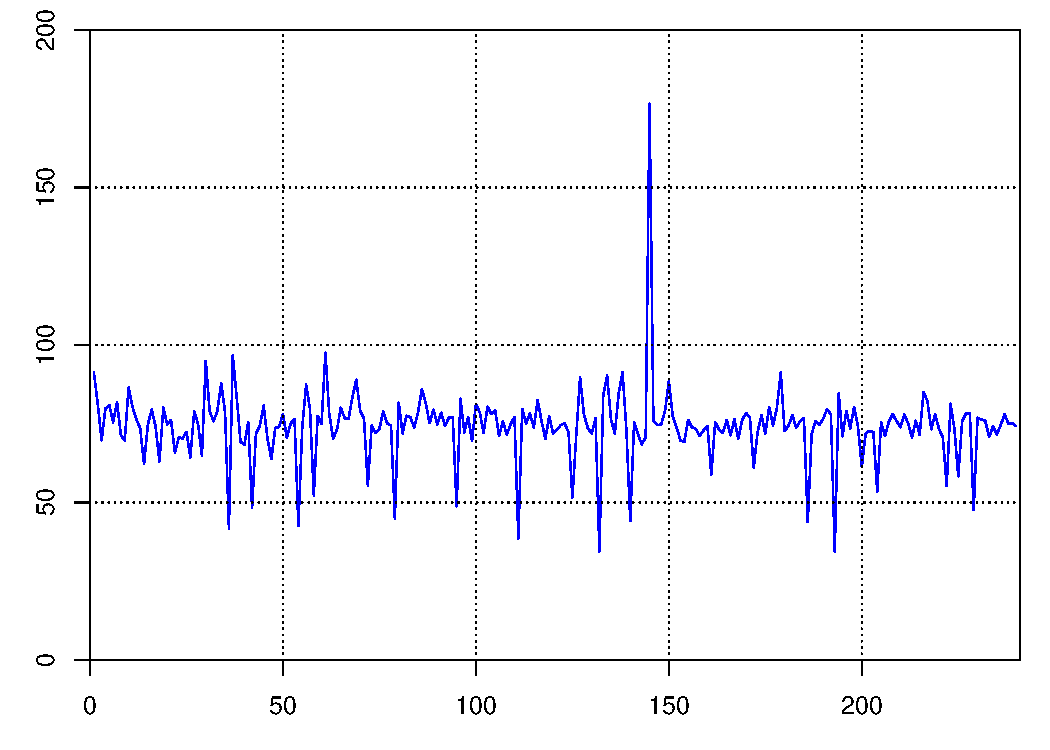
\includegraphics[width = 0.4\hsize]{aws}
}~
\subfigure[SINET ウェブサーバ]{
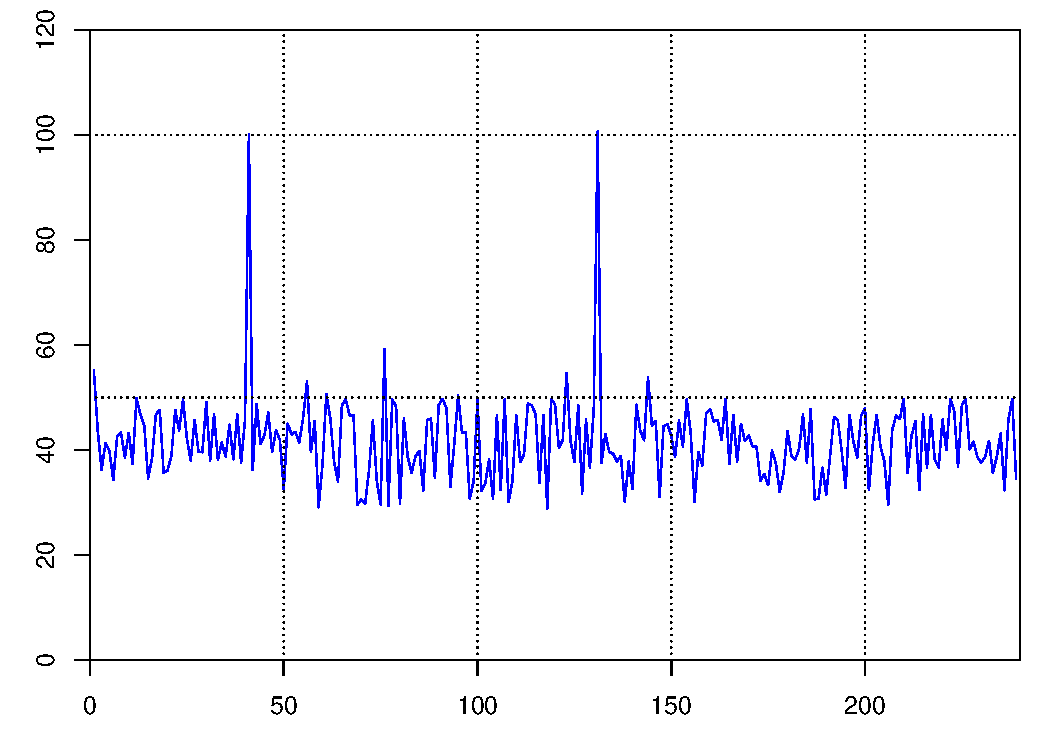
\includegraphics[width = 0.4\hsize]{sinet}
}\\
\caption{実測値の系列}
\end{figure}

\end{document}
